\chapter{Background and Motivation}
\label{chap:Intro}
\textit{The first chapter introduces fluorescence-based DNA technology and highlights the motivation of the research conducted in the thesis}
\vfill
\minitoc
\newpage

\section{Nucleic Acids}
 The nucleic acids, deoxyribonucleic acid (DNA) and ribonucleic acid (RNA), are central biological molecules in all living organisms.\cite{Bloomfield} Since the function of DNA and RNA in various biological environments are directly related to their three-dimensional structure and time-dependent structural changes (dynamics), insight into these properties is a vital requirement in order to understand genetic deceases, develop cures, exploit biological processes in various technologies, and simply to understand life itself.

 The DNA molecule is a linear polymer built up from four different subunits called nucleotides (Figure \ref{Fig:chap_intro_dna}a). Each nucleotide consists of a five-carbon, ring-structured sugar, a negatively charged phosphate group and one of the four natural nucleobases; adenine (A), thymine (T), cytosine (C) and guanine (G). The nucleobases are planar, aromatic, heterocyclic compounds capable of forming highly specific H-bonds to their complementary counterpart (A to T and C to G). Through base-pairing, two complementary strands of DNA may be hybridized resulting in a DNA duplex of two antiparallel strands and a net negative charge. DNA duplexes may adopt a number of different conformations, of which the most stable form at biological conditions is the famous B-DNA double helix (Figure \ref{Fig:chap_intro_dna}b).\cite{Watson1953} In B-DNA the base pairs are located in a hydrophobic core while the backbone is exposed on the outside of the helix where the negative charges are neutralized by counter ions in the solution. The B-DNA helix is right-handed with a helical twist of $\sim$36$^\circ$ per base pair, and an average of $\sim$10.5 base-pairs per turn corresponding to a distance of 3.4 nm. Alternative DNA conformations such as triplexes \cite{Felsenfeld1957,Duca2008} and G-rich quadruplex structures \cite{Davis2007} also exist. The role of these more complex structures in chromosomal DNA have recently received attention since they may serve as targets for therapeutic drugs.\cite{Jain2008,Chin2007,Besch2004,Huppert2008,Qin2008,Chen2008} The role of RNA enzymes (ribozymes) and switches (riboswitches) has also received attention due their role in \emph{e.g.} gene control.\cite{Serganov2007}

\begin{figure}
    \centering
        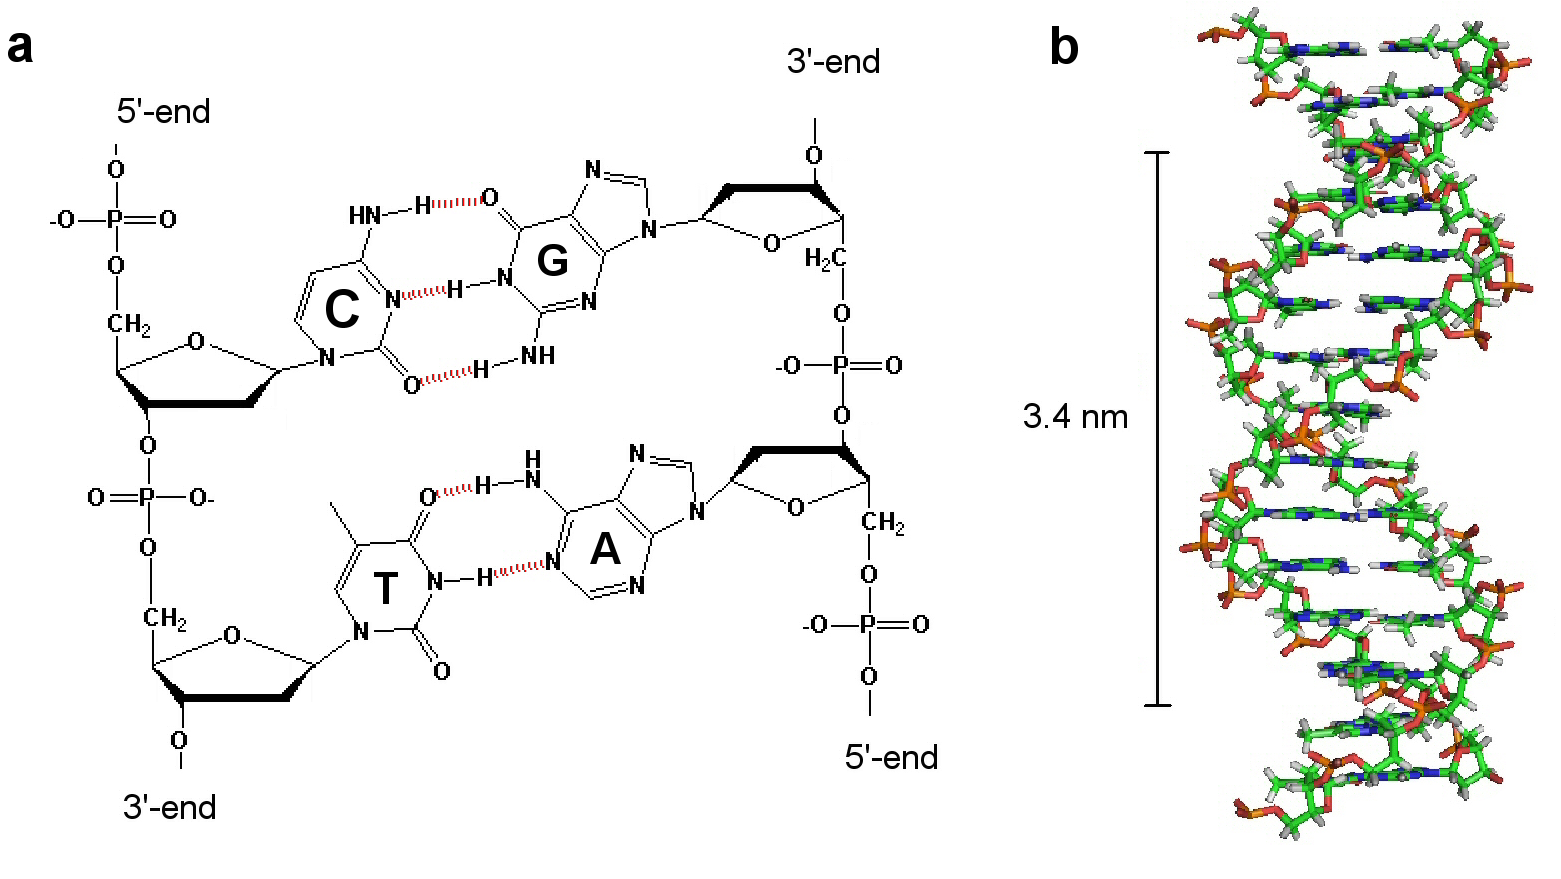
\includegraphics[width=0.88\textwidth]{adds//dna.png}
    \captionsetup{width=.95\textwidth}
    \caption{The DNA molecule. a) The chemical structure of DNA in which all four canonical nucleotides are shown in their base-pairing environment. b) The double-stranded B-DNA helix consisting of two antiparallel DNA strands hybridized as a result of Watson-Crick H-bonding between complementary bases in the two strands.}
    \label{Fig:chap_intro_dna}
\end{figure}

 The high specificity of Watson-Crick hydrogen bonding allows DNA molecules to be taken out of their biological context and exploited as building blocks in the construction of self-assembled nanoscale structures and functional devices (for recent reviews see e.g. \cite{Seeman2007,Seeman2010,Kuzuya2010,Nangreave2010,Torring2011,Shih2010,Aldaye2008}). The rigidity and chemical stability of the B-DNA helix makes this self-assembly approach highly attractive, in particular because it is relatively easy to design intermolecular nanostructures with predefined 2D- and 3D-shapes \cite{Tumpane2007,Rothemund2006,Simmel2008,Dietz2009,Douglas2009} and even a functionality such as mechanical movement \cite{Shin2004,Chen2004,Sherman2004,Li2002,Wickham2012,Wickham2011,Lund2010}, catalytic activity \cite{Baum2008,Chen2004a,Xiao2004} or drug transport\cite{Andersen2009,Douglas2012}.

\section{Fluorescence and Nucleic Acids}
 Over the years, fluorescence-based techniques have become invaluable tools in the molecular biosciences, and several new classes of fluorescent probes have recently been created to study biomolecules. The main advantage of fluorescence-based methods is that the natural nucleobases are virtually non-fluorescent \cite{Callis1983} enabling an outstanding signal-to-noise ratio when introducing fluorescence into DNA.

\subsection{Biocompatible Fluorescent Dyes}
 Fluorescent dyes may be introduced into DNA either non-covalently or covalently. Non-covalent DNA-binding dyes such as ethidium bromide bind to DNA by unspecific electrostatic interactions with the negatively charged backbone and/or by intercalation in between the hydrophobic bases.\cite{Ihmels2005,Armitage2005} In contrast, covalently attached fluorophores are usually tethered via a flexible linker to the DNA. This approach allows practically any fluorophore to be attached to the DNA at several different sites. The most popular probes are commercially available dyes such as the Cy-dyes and the Alexa-dyes which offer an unsurpassable overall brightness. These dyes are available in a variety spanning the entire visible spectrum.\cite{lifetechnologies} Alternative luminescent probes are e.g. lanthanides characterized by long excited state lifetimes\cite{Selvin2002} and inorganic semi-conductor quantum dots\cite{Giepmans2006,Medintz2005} characterized by their extremely high brightness.

 Using dyes attached externally to biomolecules has a number of disadvantages. Firstly, dyes often interact with their surrounding environment which may hamper the interpretation of experiments or change the fluorescence properties of the dye.\cite{Iqbal2008a,Neubauer2007,Norman2000,Sanborn2007,Sabanayagam2005a} Secondly, since external dyes reside on the outside of the biomolecular surface there is an inherent limitation in the kind of information obtainable from quantitative fluorescence experiments since the probes respond and report indirectly on the structure and dynamics of the biomolecule.

\subsection{Fluorescent Nucleobase Analogues}

 For studies involving nucleic acids, fluorescent nucleobase analogues constitute a different class of fluorophores that overcomes these problems (for reviews see \cite{Wilhelmsson2010,Sinkeldam2010,Rist2002,Hawkins2003,Okamoto2005,Wilson2006,Asseline2006,Loakes2007}). These probes can be inserted into DNA as a replacement for one of the natural bases mimicking the properties of the substituted base, in most cases without significantly affecting the DNA structure and function. In addition, when using nucleobase analogues the reporter can be positioned close to or even in the very site of interest when investigating DNA. Traditionally, the most utilized fluorescent nucleobase analogue has been 2-aminopurine (2-AP), an isomer of adenine capable of forming a base-pair with thymine and a less stable base-pair with cytosine.\cite{Freese1959} 2-AP is highly fluorescent in its free, monomeric form but is almost completely quenched in the base-stacking environment provided by dsDNA.\cite{Ward1969} This property has been exploited in probing the local structure and dynamics of DNA \cite{Guest1991,Xu1994,Millar1996} and in DNA-protein interactions that result in locally unwound strands \cite{Millar1996,Hochstrasser1994,Raney1994}. Other reported fluorescent base analogues include, but is not limited to, the pteridines\cite{Hawkins2001}, the expanded DNA bases\cite{Liu2004}, the wide DNA bases\cite{Lu2004}, the base-discriminating fluorescent base analogues\cite{Okamoto2003,Okamoto2003a,Okamoto2003b,Okamoto2005} and the emissive RNA alphabet by Tor and co-workers\cite{Shin2011}.

 The strict environment set by the DNA double helix in terms of H-bonding, base-stacking and steric hindrances, however, often affects the fluorescence properties of the fluorophore. As a result, fluorescent nucleobase analogues lag behind commercially available dye molecules in terms of overall brightness and spectral properties. Developing new fluorescent base analogues thus remains somewhat challenging. Common for all the fluorescent nucleobase analogues mentioned above are their sensitivity to the surrounding micro-environment, most often a significant quenching of fluorescence in dsDNA and a strong destabilizing effect of the DNA double helix. The highly relevant exception to these properties is the tricyclic cytosine (tC) family, 1,3-diaza-2-oxophenothiazine (tC), 1,3-diaza-2-oxophenoxazine (tC$^\mathrm{O}$) and 7-nitro-1,3- diaza-2-oxophenothiazine (tC$_\mathrm{nitro}$).\cite{Wilhelmsson2010,Wilhelmsson2001,Wilhelmsson2003,Sandin2005,Sandin2007,Sandin2008,Engman2004,Borjesson2009a,Preus2010} These base analogues are directly built upon the molecular framework of cytosine and extended by two extra rings (Figure \ref{Fig:chap_intro_tcprobes}). tC and tC$^\mathrm{O}$ both possess high fluorescence quantum yields ($\sim$0.2) and single-exponential lifetimes ($\sim$4-5 ns) in double-stranded DNA, relatively insensitive of neighbouring bases.\cite{Sandin2005,Sandin2008} In contrast, tC$_\mathrm{nitro}$ is virtually non-fluorescent at room-temperature but possess a red-shifted lowest energy absorption band compared to tC and tC$^\mathrm{O}$ which makes it perfectly suited as an energy transfer acceptor with tC or tC$^\mathrm{O}$ serving as the donor (Figure \ref{Fig:chap_intro_tcprobes}).\cite{Borjesson2009a,Preus2010} All of the tC probes adapt the position and orientation of the substituted cytosine base and stabilize the B-DNA double helix compared to regular cytosine.\cite{Engman2004,Sandin2008,Borjesson2009a}

 The tC family has a central role in this thesis. In Paper II and V they are subjected to a thorough photophysical characterization, while Paper III demonstrates their use in probing DNA structure and dynamics.

\begin{figure}
    \centering
        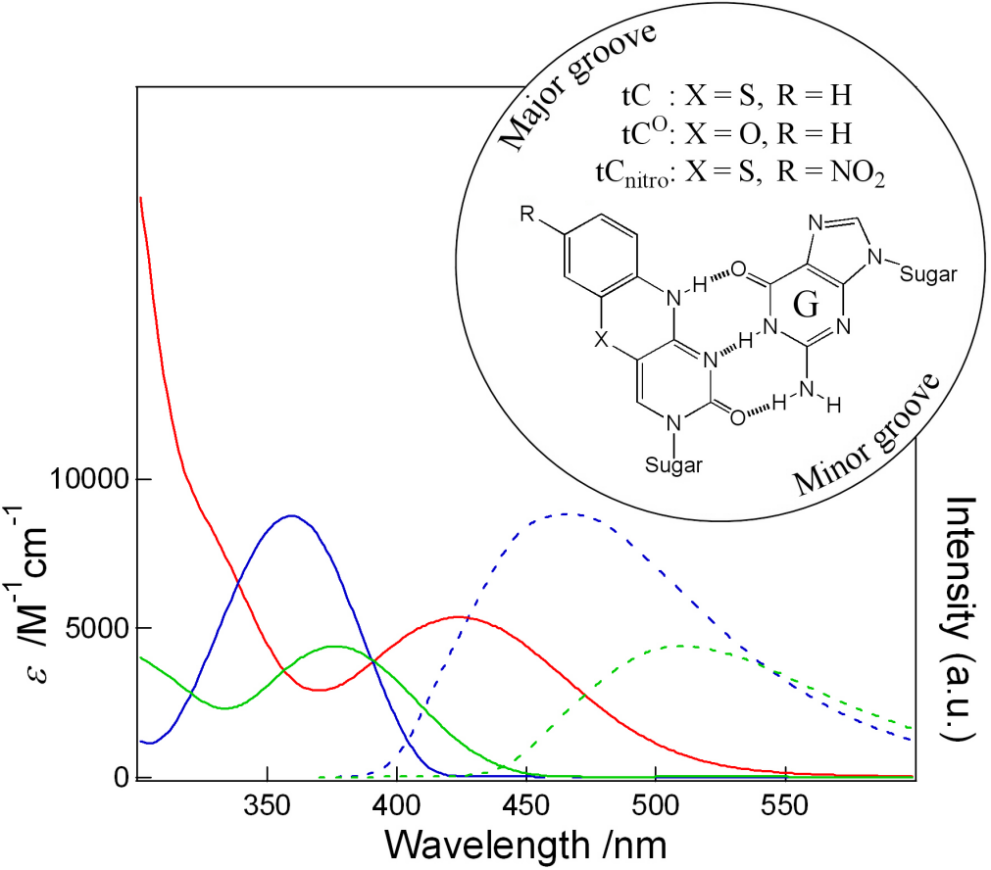
\includegraphics[width=0.65\textwidth]{adds//tcprobes.png}
    \captionsetup{width=.95\textwidth}
    \caption{UV-Vis absorption (full-drawn) and emission spectra (dashed) of the tricyclic cytosine analogues, tC (green), tC$^\mathrm{O}$ (blue) and tC$_\mathrm{nitro}$ (red). Insert: Chemical structures of the tC probes in the base-pairing environment with guanine.}
    \label{Fig:chap_intro_tcprobes}
\end{figure}

\subsection{FRET and Nucleic Acids}
 FRET is an energy transfer phenomenon that is widely used as a molecular ruler in the biosciences for probing nanoscale distances and molecular interactions (Figure \ref{Fig:chap_intro_fret}).\cite{Lak} The technique is usually performed by covalently labelling one or more biomolecules with two dyes: an energy donor and an acceptor. If the two probes are located within a distance related to the critical Förster distance of the pair (<10 nm) energy transfer can be induced between the two dyes which is observed as a decreased donor fluorescence yield, decreased donor excited state lifetime and, if the acceptor is emissive, an increased acceptor fluorescence yield. FRET may thus either serve as an "on/off" sensor of the relative location of the two dyes or as a quantitative ruler for determining the distance in between the FRET-pair. One of the aims of this thesis is to demonstrate that much more quantitative information, than a mere relative distance, can be gained from FRET experiments.

\begin{figure}
    \centering
        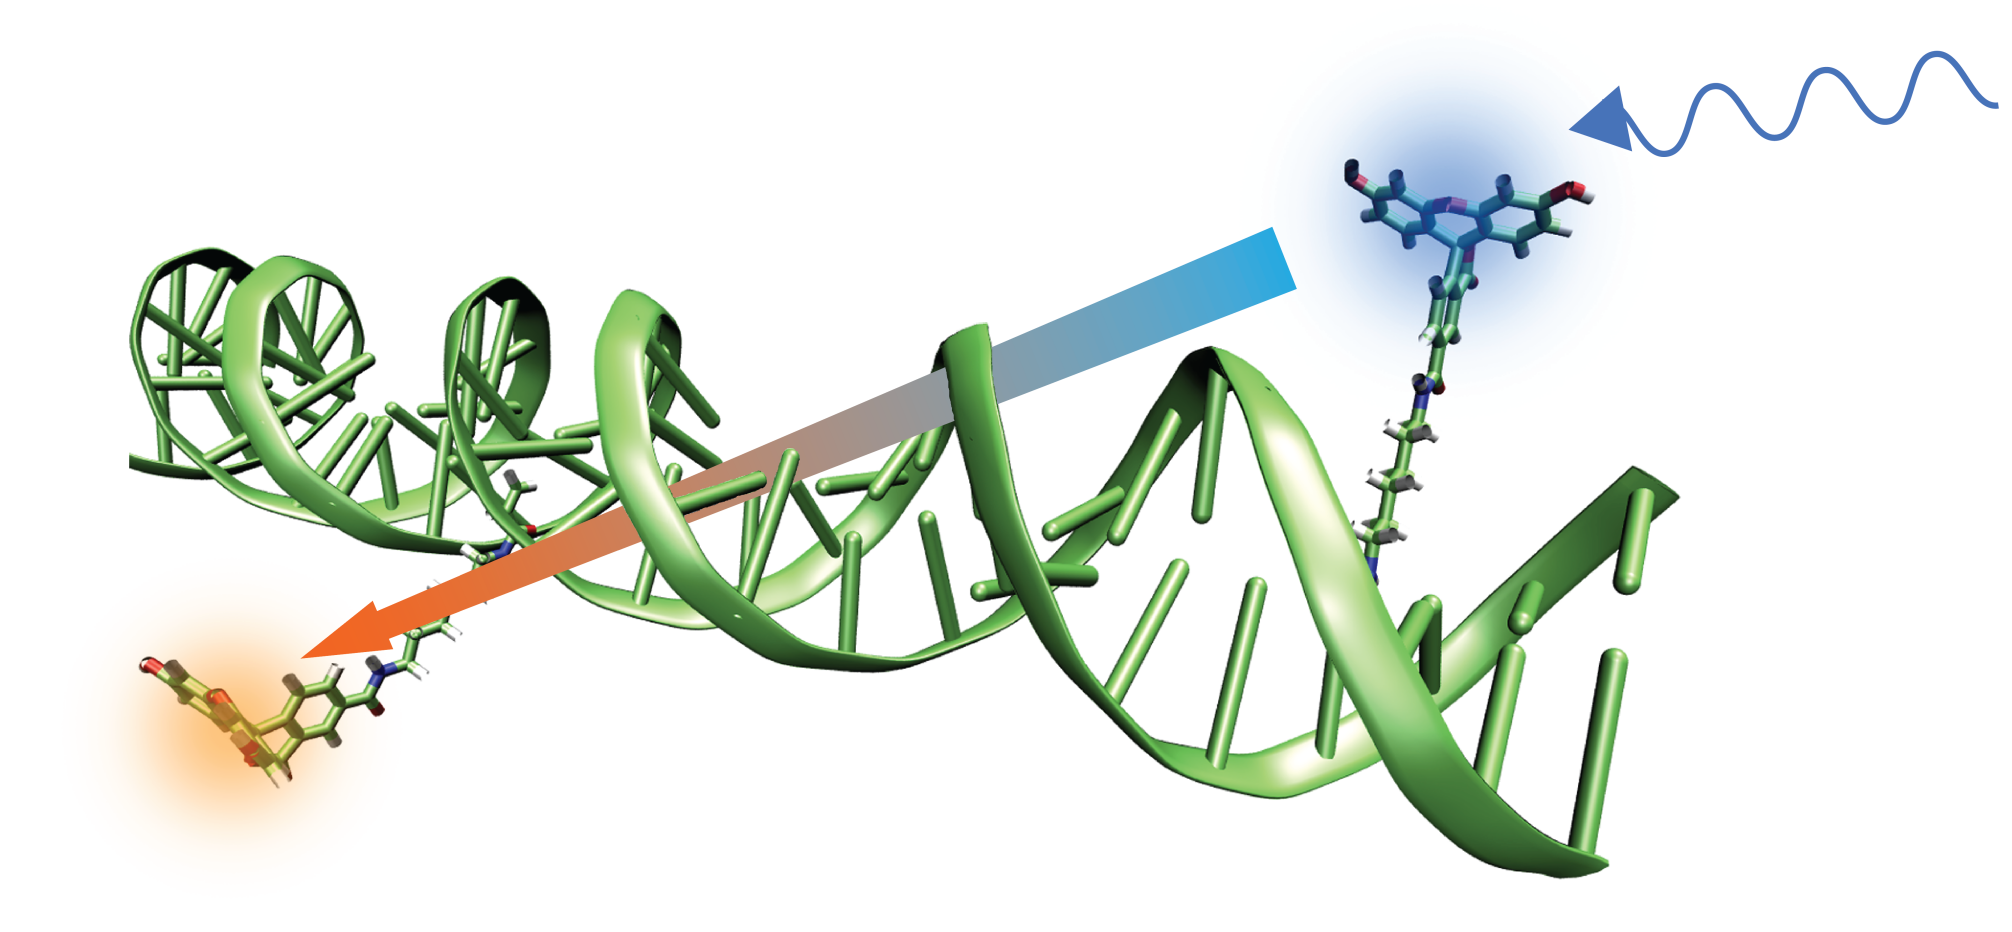
\includegraphics[width=0.8\textwidth]{adds//fret.png}
    \captionsetup{width=.95\textwidth}
    \caption{Illustration of FRET between two dyes tethered to DNA. After excitation of the donor this dye transfers its excitation energy to the acceptor located in close proximity. The FRET efficiency is highly distance dependent which makes the technique suited as a "molecular ruler" for probing nanoscale distances and molecular interactions.}
    \label{Fig:chap_intro_fret}
\end{figure}

\subsubsection{Historical View}
 FRET was first described by Förster in the 1940's as an interaction between two dipoles separated by a fixed distance, $r$, and oscillating in resonance.\cite{Foerster1948} By multiplying the probability that the two dipoles have the same resonance frequency with the rate of energy transfer when they do have the same resonance frequency, Förster derived the characteristic $r^{-6}$ dependency of the energy transfer rate constant (section \ref{sec:FRET}).\cite{Clegg1996} The FRET theory was continued to be discussed up to and during the 1970's\cite{Stryer1967,Dale1974,Dale1979}, however, it was not until late 1980's and early 1990's that FRET was exploited as a quantitative ruler to probe distances within nucleic acid structures.\cite{Murchie1989,Clegg1992b} In these studies, Lilley and co-workers determined the stereochemical arrangement of the four helices making up the Holliday junction, a four-stranded, four-way DNA junction which is an intermediate in genetic recombination. This late entrance of quantitative FRET in DNA was mainly due to difficulties in labeling nucleic acids site-specifically at that time. However, the DNA fluorescence toolbox has advanced greatly since then and custom dye-labelled oligonucleotides are now ordered and delivered on a day-to-day basis.\cite{lifetechnologies,GEHealthcare,GlenResearch,IDT,atdbio}

\subsubsection{FRET in Modern Applications}
 Today, FRET is used routinely as a technique to probe the structural states of nucleic acids. Particular advancement has occurred in recent years in the specific case where quantitative information about FRET-pair distances and nucleic acid three-dimensional structures is wanted from FRET experiments. The combination of multiple FRET-pair positions has provided quantitative insight into the three-dimensional structure of nucleic acids.\cite{Muschielok2008,Muschielok2011,Sabir2011,Sabir2012,Wozniak2008,Andrecka2008,Andrecka2009,Balci2011} Increasingly sophisticated techniques have been developed to model the uncertainty in the position and orientation of the dyes relative to the DNA.\cite{Muschielok2008,Sindbert2011,Rindermann2011} In addition to these improvements, the properties of many popular commercial FRET dyes attached to DNA are now known to some extent, such as the Cy-dyes\cite{Levitus2011,Norman2000,Sanborn2007,Iqbal2008a,Harvey2009,Harvey2009a}, FAM\cite{Noble2005,Unruh2005,Unruh2005a,Wang2004} and TAMRA\cite{Unruh2005,Unruh2005a,Wang2004,Vamosi1996,Stennett2012}. This knowledge is not only insightful but in fact vital in order to use FRET quantitatively on nucleic acid containing systems.

 An exciting development within FRET is the ability to monitor one molecule at a time, called single-molecule FRET (smFRET).\cite{Mollova2002,McKinney2004,Selvin2008,Roy2008,Joo2008} Single-molecule FRET techniques provide real-time insight into biomolecular structures and dynamics without hiding molecular heterogeneity behind an ensemble average. However, interpreting smFRET experiments into quantitative distances and dynamics is extremely difficult due to the low signal-to-noise ratio in such experiments, and methods are still being developed for analysing data from smFRET experiments quantitatively.\cite{Watkins2006,Gopich2005,Gopich2007,Gopich2009,Nir2006,Antonik2006,Kalinin2008,Kalinin2010} Multiparameter single-molecule fluorescence techniques, in which all possible ascertainable fluorescence parameters are monitored at the single-molecule level (intensity, anisotropy and lifetime), are extremely interesting in the context of quantitative smFRET.\cite{Sisamakis2010,Kuhnemuth2001,Kudryavtsev2012,Eggeling2006,Widengren2006,Laurence2005,Muller2005} Because all information required to interpret the measured signal into quantitative distances are acquired, such state-of-the art single-molecule techniques offer vast potential for providing detailed insight into the structure and dynamics of large biomolecules. Recently, single-molecule FRET has been used to probe the three-dimensional geometry of three-way DNA junctions\cite{Sabir2011,Sabir2012}, RNA polymerase II complexes\cite{Andrecka2008,Andrecka2009,Treutlein2012} and a helicase-DNA complex\cite{Balci2011} to name but a few.

 More references and information on recent advances within quantitative FRET is found in Paper I of this thesis.

 \paragraph{Base-base FRET.} In a previous study of ours (Appendix 1), a fluorescent nucleobase analogue FRET pair system was developed as an alternative to traditional, external FRET probes (Figure \ref{Fig:chap_intro_basefret}).\cite{Borjesson2009a} Since the base probes adapt the position and orientation of the canonical bases within double-stranded DNA this technique provides a number of advantages compared to traditional probes: First of all, the base probes can be positioned inside the very site of interest mimicking the behaviour of the substituted base and, thus, provides a means to probe the local base orientation and position at specific sites. Secondly, because both the orientation and position of the probes are highly constrained at the timescale of energy transfer this allows a higher degree of control of the orientation factor in the energy transfer process, and thus more detailed studies to be performed of three-dimensional nucleic acid structures without complications associated with linker flexibility.

 This latter point is demonstrated by the FRET efficiencies measured between the base analogue FRET-pairs positioned in B-DNA with distances varying from 2-13 base-pairs in between the FRET-pair (Figure \ref{Fig:chap_intro_basefretgraph}).\cite{Borjesson2009a} As the number of bases in between the pair increases both the distance as well as the relative orientation between the donor and acceptor gradually changes in a predictable manner. The result is a FRET curve decreasing with distance and, additionally, oscillating with a periodicity in phase with the helical periodicity of the B-DNA helix due to the change in orientation between the two transition dipole moments of the probes. The oscillation of the measured energy transfer efficiency in Figure \ref{Fig:chap_intro_basefretgraph} demonstrates the well-defined orientation of the base probes inside the DNA helix. The main disadvantage of base-base FRET is the complexity involved in the quantitative analysis of data from such experiments. A solution to this limitation is provided in this thesis.

\begin{figure}
    \centering
        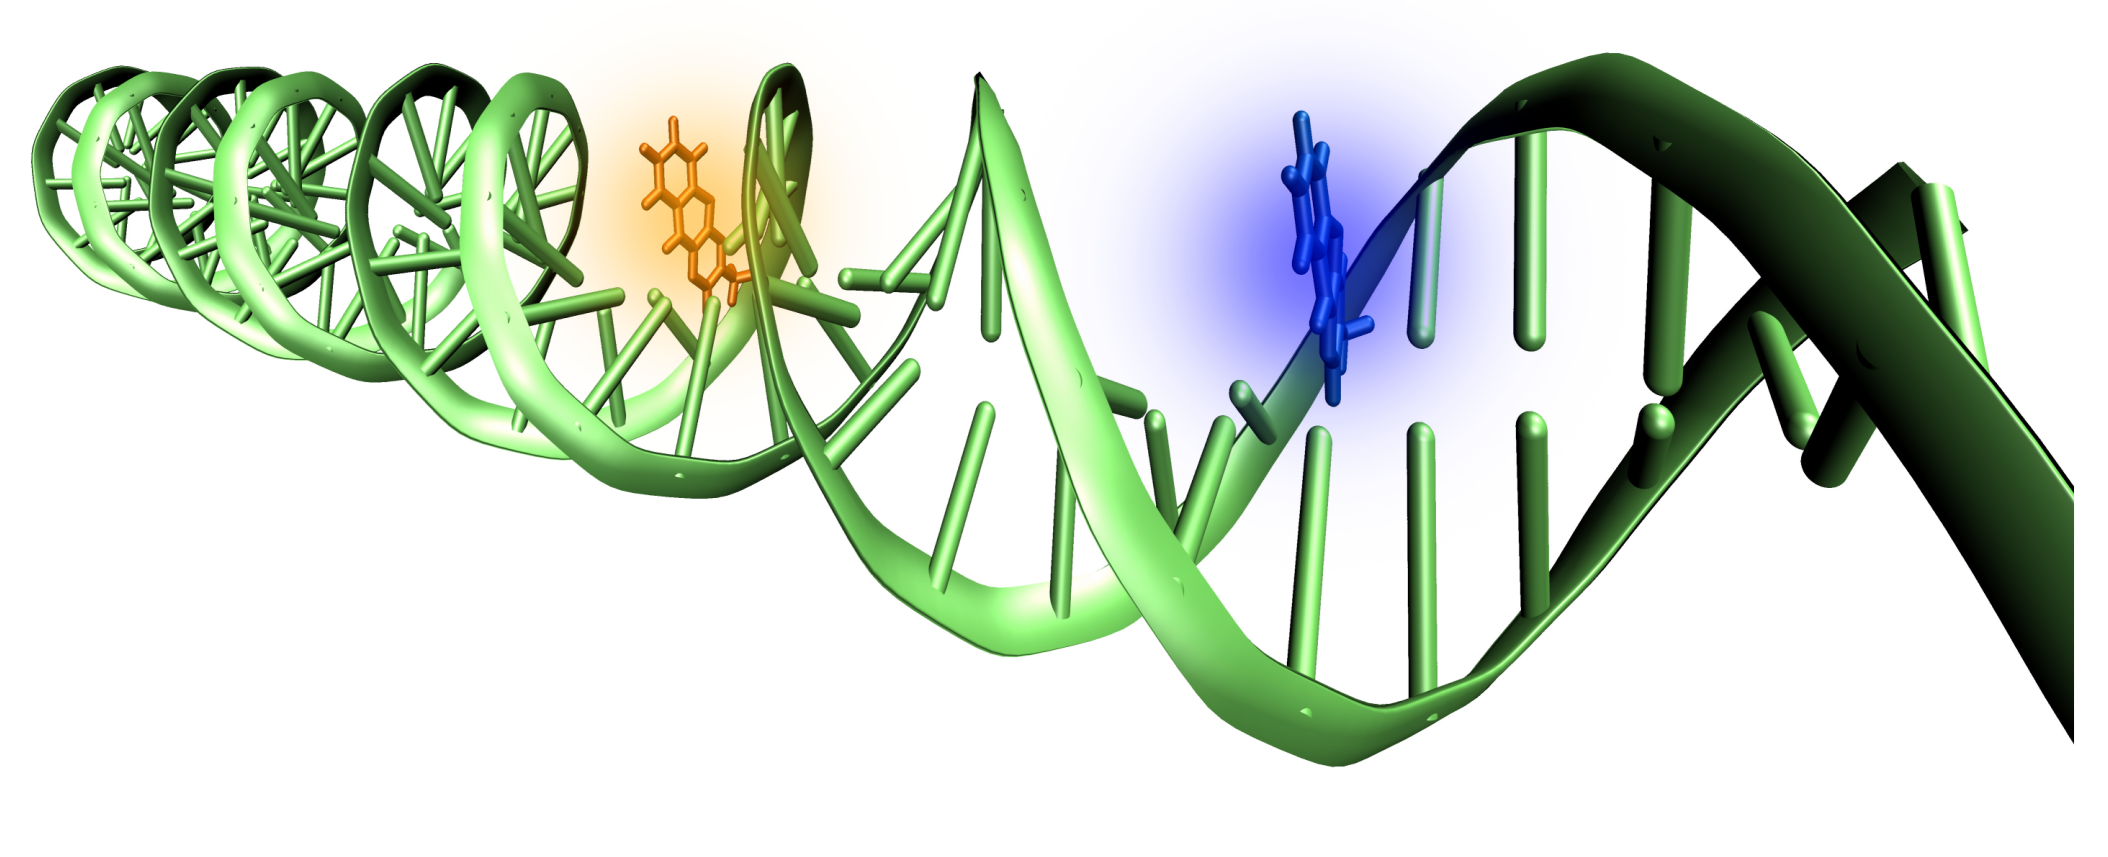
\includegraphics[width=0.7\textwidth]{adds//basefret.png}
    \captionsetup{width=.95\textwidth}
    \caption{Illustration of two base analogues positioned in B-DNA providing the foundation for base-base FRET.}
    \label{Fig:chap_intro_basefret}
\end{figure}
\begin{figure}
    \centering
        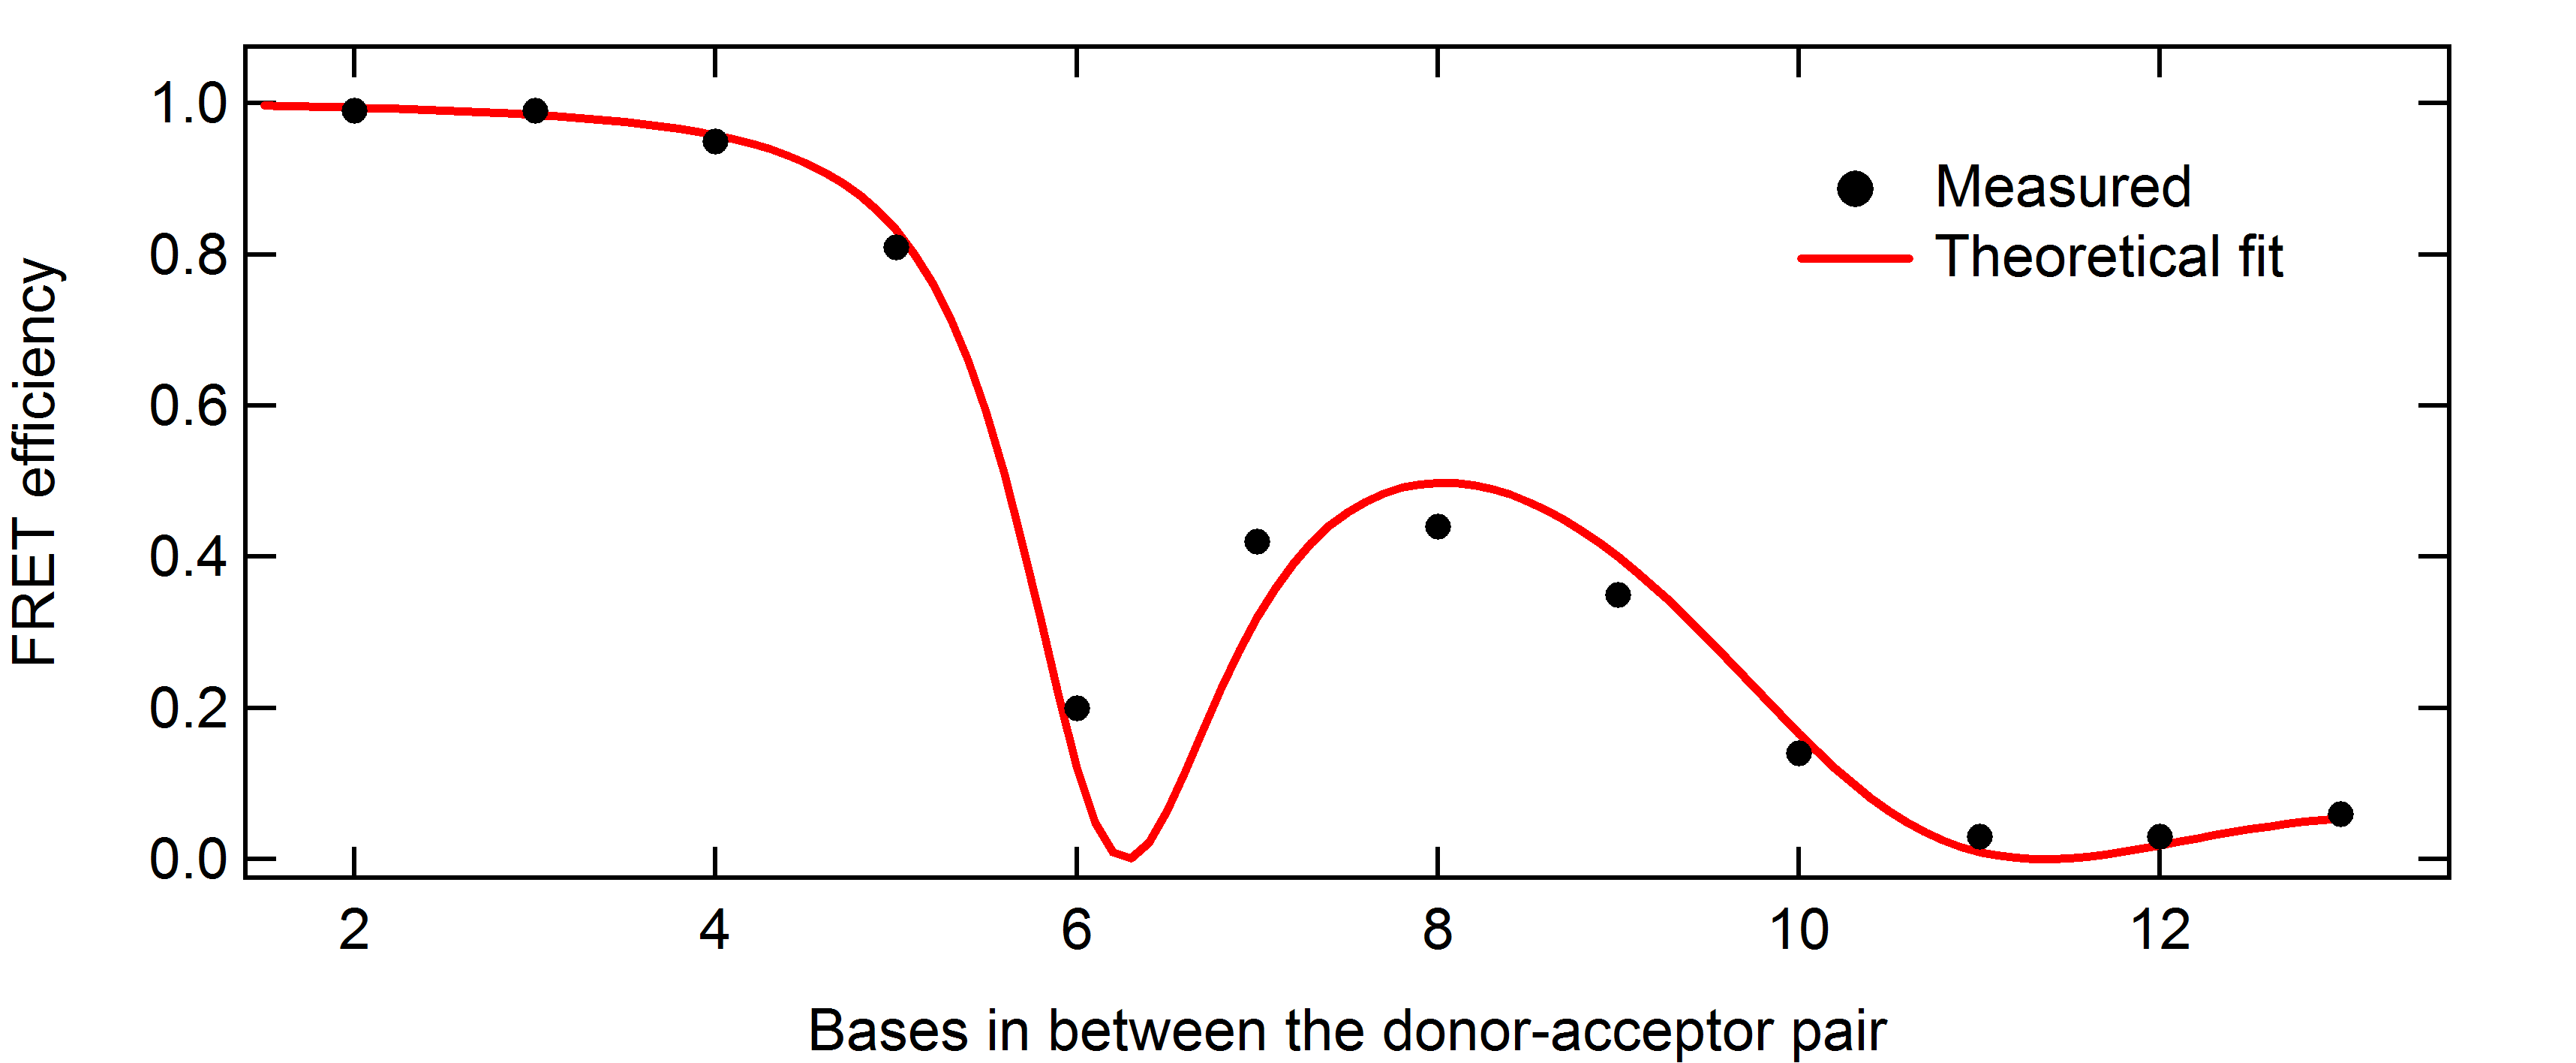
\includegraphics[width=0.7\textwidth]{adds//basefretgraph.png}
    \captionsetup{width=.95\textwidth}
    \caption{The FRET efficiencies measured between two base analogues positioned inside double-stranded B-DNA with varying inter-pair distance.\cite{Borjesson2009a} The red line is a theoretical fit based on the assumption of static transition dipoles positioned inside a perfect B-form helix with a twist of 36$^\circ$ and rise of 3.4 Å per dinucleotide step.}
    \label{Fig:chap_intro_basefretgraph}
\end{figure}

\subsubsection{Advantages and Drawbacks}
 Compared to higher resolution structural techniques like NMR spectroscopy\cite{Foster2007} and X-ray crystallography\cite{Holbrook2008}, FRET has the advantage of not being limited by the size of the system under investigation (unlike NMR), is solution-based (unlike crystallography) and, in addition, FRET is generally cheaper, faster, simpler and more sensitive. The drawbacks of FRET, however, are the dependency of the energy transfer on 1) probe orientation, which is very hard to control, and 2) the fluorescence quantum yield of the donor, which strongly depends on the interaction between the probe and its micro-environment and thus vary from sample to sample. While the second drawback can be accounted for using proper reference measurements (i.e. by using reference samples labelled with the donor only) the first drawback is more difficult to account for. Lower and upper boundaries of $\kappa^2$ can be estimated based on fluorescence anisotropy measurements\cite{Dale1974,Dale1979}, however, the exact $\kappa^2$-value or $\kappa^2$-distribution is practically impossible to obtain. This problem leads to an uncertainty in the distance deduced from FRET measurements.

 In this thesis, the novel FRET technique base-base FRET is developed and refined. It is demonstrated how the method facilitates an unprecedentedly high control of the position and orientation of the FRET probes and thus leads to more accurate and versatile quantitative FRET-based experiments.


